\documentclass[a4paper]{article}
\usepackage[english]{babel}
\usepackage[utf8x]{inputenc}
\usepackage[margin=1.0in]{geometry}
\usepackage{amsmath}
\usepackage{graphicx}
\usepackage[colorinlistoftodos]{todonotes}
\usepackage{graphicx}
\DeclareGraphicsExtensions{.pdf,.png,.jpg}
\title{CS240: Individual Report}
\author{Vikram S. Nilakantan, Graham Baker, Walker Bohannan, Jessica Penick, Steve Marx, Eli Spiegel}
\begin{document}
%-------------------------------------------------------------------------------------------------------------
% TITLE PAGE
%-------------------------------------------------------------------------------------------------------------
\begin{titlepage}
\vspace*{\fill} %leave out given vertical space in a document
\begin{center}
{\Huge Visual Editor Final Report}\\ [0.5cm] 
%make title huge and have .5cm space in between
{\Large Graham Baker, Walker Bohannan, Jessica Penick, \\Steve Marx, Vikram Nilakantan, Eli Spiegel}\\[0.4cm]
\today %put the date that the data is compiled
\end{center}
\vspace*{\fill}
\end{titlepage}
\section{Project Summary}
Edith is educational software designed to introduce new computer science students to programming. New students of any age can learn basic object-oriented programming concepts prior to learning a particular programming language in detail (syntax, data types and structures, etc.). Edith provides a graphical user interface through which users can create a ``script" that animates 2-D characters, or sprites, provided by the program or loaded and created by the user. The user creates the script by piecing together provided blocks of program structure in a functional way. Similar programs (e.g., Alice, Scratch) have been shown to increase the interest level and retention of students taking their first programming classes. Edith is written primarily in JavaScript and is available over the Internet. The software is expected to be open-source to allow further development and additional educational opportunities. \newline \newline 
The first step for the user of Edith is to create an account by entering a user name and password. With the account, the user can save projects and come back to work on them later, or share projects with friends and classmates. After an account is created (or a user logs in to an existing account), Edith also allows the user to either select an existing sprite, load a new sprite from a file, or create (draw) his own character within the program by selecting ``Make Object." Even new computer users will be able to make simple objects using the provided shapes and drawing methods. \newline \newline 
The Visual Editor (VE) module provides a visual programming language editor (in essence, an integrated development environment(IDE)). The user selects a sprite(s) to be added to the canvas and be animated, and the VE allows users to arrange programming elements to create an animation sequence. VE programming elements are contained in three categories, accessed through one of three drop-down boxes. The first category, ``Method", allows the user to define methods and variables, and includes and end block for the program. The second category, ``Predefined", includes given methods that the user can easily apply to sprites (wait, rotate, move, jump, move right, move left, move up, move down). The final category, ``Control", provides if, while and else blocks for the user's animation. The user creates the animation by selecting from the available VE blocks and dragging them to the right of a line to the code sequence area. When a block is dragged to the code sequence area, the user will be prompted for appropriate inputs (e.g., variable names, or the distance for the sprite to move). User inputs are checked for type; if a user enters a word rather than a number for distance moved, the user will be prompted again for a number. Blocks can also be dragged from the code sequence area back to the main VE option area; this removes that section of code in real time. As the user is creating the block of code, the VE, while enforcing syntax rules, converts the program into JavaScript to be executed. Upon creation of an animation sequence, the user will not need to wait for compiling to see if the code ``works". Rather, the code, or sequence of events defined by the user, will be always ready to run (``play") unless a script notifies the user otherwise.
\section{Development Procedures}
Incremental development (a fundamental part of agile approaches) was used to develop the Visual Editor module. This general method of development made sense for the Edith project, as the team needed to move toward a solution in a series of incremental steps. Given that the languages and technologies were new to the team members, it was the only option for development process. The team did not know enough to plan everything at the beginning, and needed to build on successive iterations that added functionality and got closer to the objectives. Not surprisingly, as the VE team began its work and planning on the project, which development procedure would be used was not a topic of discussion or debate. It should be noted that with more software project experience, project management experience, and with the benefit of more time, additional early planning about how teams are going to go about a project could pay great dividends. \newline \newline 
The VE team's development methodology could accurately be classified as Rapid Application Development (``RAD"). RAD was a natural fit for the VE portion of Edith, as prototypes needed to be developed quickly, with additional functionality and interaction with other modules added for each integration date in the project schedule. One weakness of RAD and related methodologies is reliance on communal decision-making processes. In Edith, there was ongoing confusion on the purpose and role boundaries between VE and other modules; this confusion was not resolved for many weeks. Meanwhile, the VE team assigned some functionality to its team members, and excellent individual efforts produced various early prototypes. One issue was that there were still different ideas about what the module should do, far beyond how it should be done, and it took a lot of time to get to the point where the team was building on the same prototype. This may have been resolved with earlier team integration and collaboration as a mutual understanding and method of development were being formed. However, once more advanced prototypes were being developed, it became easier to combine desirable elements of various prototypes. \newline \newline 
The order of component development is difficult to state precisely, as many components were being worked on concurrently. In basic order: creation of blocks; adding text to blocks; cloning blocks; dragging and dropping blocks; getting user input when blocks are dropped; sorting based on the y positions of the boxes; user input verification. \newline \newline 
Testing was performed primarily by the VE team testing the software from the user's perspective. This natural testing method was very effective and provided direction for program correction and feature improvement. Static analysis was performed midway through development, but at that point it did not offer much insight, as the code did not have specific errors to be caught by static analysis, and the tools seemed to offer more style than substance feedback.\newline \newline 
Some of the contributions of VE team members include: \newline \newline 
Graham Baker - made the sorting function that reads the y positions of the boxes, gets their ids, then puts them all in a string to give to animation. Also made the tabs and helped with save and load functions. Got all of the functions from animation and put them into boxes and made prompts to fill the attributes. \newline \newline 
Walker Bohannan - was responsible for most of the functionality with the double-click, drag-start, drag-end functions. He was also co-responsible for the saving and loading of JSON code so blocks can be put into the canvas again, and helped implement cancelling of boxes, as well cloning when dragged over the line. In addition helped implement the grouping of text and rectangle objects with auto-height and -width functionality. \newline \newline 
Steve Marx – added user input checks using regex so that variable names, method names, and predefined method inputs make/prompt user to enter the right type of data. Worked on some JSON issues. \newline \newline 
Vikram Nilakantan - was responsible for working on the block dynamic creation. AJAX server syncing (used by sharing framework, story creator, and object team) as well as loading and saving VE method blocks.\newline \newline 
Jessica Penick - worked on commenting code, cloning and intergroup relations.\newline \newline 
Eli Spiegel – wrote a majority of first two integrations getting blocks that could drag and drop and being able to have user input as those blocks got dropped. Later in the project continued to work with Vikram, Graham, and Walker on the code but also moved to working more with other teams as to find how we could integrate with them. For one of the biggest pieces of integration worked with Eric Lund to get it so VE blocks could add sprite and actually animate them; helped him understand VE code and worked to help him find a solution for how VE blocks could call their methods with the objects Object Team had created.\newline \newline 
\section{Requirements Evaluation}
Non-Functional Requirements and their Status: \newline \newline 
1) Usability. (Training should not be required for users to effectively use the module. 
Module documentation and basic age-specific computer knowledge should provide sufficient guidance.
The module should allow the user to recover from errors with informative and understandable error messages.) Partially met - Training is not required, but documentation should be improved to facilitate module use. Input error messages allow users to recover from some errors, but more help, tips and code issue checking would improve usability. \newline \newline 
2) Documentation. (The module will provide documentation that allows users to easily begin using the system.) Partially met - At this point, it does not seem that users can ``easily" begin using Edith. More extensive instruction should be provided on how to get started, drag and drop blocks, etc. \newline \newline 
3) Modifiability. (The module will have the flexibility to allow feature expansion over time.) Met - Additional predefined methods, math, etc. can be easily added. \newline \newline 
4) Privacy. (The user's work will remain private/secure unless the user chooses to share it.) Met - The Edith site is secure and requires a username and password to access work. \newline \newline 
5) Student Learning Experience. (In order to support the learning of young computing students, the module will provide an engaging interest that increases their interest in the subject. Effectiveness may be measured by student retention rates and self-reported interest levels.) Met - the module provides the basic template to facilitate student's understanding of code structure and its effects. Additional options and refinement could further increase interest. \newline \newline 
6) Platform. (Users will be able to run the module from Windows or Mac.) Met - All of Edith can be accessed from Windows or Mac computers. \newline \newline 
7) Open Source. (After initial development, the source code will be open and redistributed with improvements by anyone.) Not Met - The class is not yet at that point, as the final integration was just yesterday. Student interest will help determine whether the project is made open source. \newline \newline 
Overall, Usability, Documentation and Student Learning Experience were the most helpful non-functional requirements, as meeting these requirements together means that the project is a basic success. In other words, if aspiring programmers can understand how to use the system and have a good learning experience, the goal has been achieved. \newline \newline
Functional Requirements and their Status: \newline \newline
1) The system shall allow the user to edit a variable. Met - the user is able to use the VE to select a variable, change parameters, and save the variable in a method. \newline \newline
2) The system shall have drag and drop functionality for methods. Met - the user can create a new variable and select it, and drag and drop it in the provided boundaries. \newline \newline
3) A user shall be able to instantiate a conditional statement. Met - the user can drag and drop a conditional statement (e.g., if) and place conditions inside. \newline \newline 
4) A user shall be able to instantiate a boolean operator. Not met - due to time constraints, boolean options were not included as the most basic functionality was prioritized. \newline \newline
5) A user shall be able to connect actions (connect selected blocks together). Not met - due to time constraints, boolean options were not included as the most basic functionality was prioritized. \newline \newline
6) The user shall be able to delete a method. Met - when the user drags a method (or other) block to the left of the story line, the method is immediately deleted from the code. \newline \newline
7) The user shall be able to instantiate a loop. Met - the system provides loop blocks (e.g., while) for the user to instantiate loops. \newline \newline
8) The system will allow the user to create a new action. Met - the user can select a new method block, drag the method into the workbox, and provide arguments to create the method. \newline \newline
9) The system will allow a sprite object to be added. Met - Edith allows the addition of provided sprites, uploaded sprites, and sprites created by the user in Edith. \newline \newline
All of the functional requirements except Connecting Actions (5) are very important; they are the basic functional elements that allow users to create animations in Edith. 
\section{System Design and Architecture}
\subsection{Code Walkthrough}
Our code starts with some global declarations, including universal main, which is passed to story creator. Universal main is the string of method calls that the end-user has written. The code then defines some regular expressions that check the input from the users to ensure they are the correct data type. There is some code that animation team added that keeps track of which sprites are currently on the canvas. The array called ``tools" contains each of the available methods which come in three types: ``method," ``predefined," and ``control" (defined later). The next major part is a function called ``promptUser". This method has two more methods inside it—-``loadUpSpritesToAnimate" and ``loadSprites", both of which make sure we have a sprite selected from the object box beneath the story canvas. Then there is a series of if statements that check what kind of method has been dragged and prompt for the appropriate arguments. The regular expressions as described earlier check that these inputs are the proper types. At the end of promptUser we return a string of the JavaScript block that has been dragged over. \newline \newline 
The next big one is ``newRect" which makes the draggable boxes seen in the editor. The color of the box is based on what kind of box it is (control, method, etc). ``Predefined" boxes are method calls received from animation team; ``control" boxes are statements like if, else, and while; and all other boxes (``method" boxes) are default methods (main, etc). The method newRect then sets up the text to display on the box, followed by defining the behaviors of the box on dragstart, double click, and dragend. On dragstart the box is moved across the canvas following the cursor. If the box has not been dragged across the threshold line (created later) before, it's cloned, if it doesn't cross the threshold line, the box gets deleted. Double click only applies to boxes that have been defined as ``sortable" (which happens when the box is cloned, since this means it is a box the user has created). Once defined ``sortable", we prompt the user, update the text and the size of the box based on the text, allowing users to change their previously generated method calls. Behavior on dragend does a lot of the same things: set the position, check if it has been dropped across the line, if it has been we prompt for parameters again, elsewise the box is deleted. We once again use the ``sort" method and set it so that it knows that it has been cloned.\newline \newline 
The next important section prepares the stage and the threshold line, which acts as a visual marker for the division between the ``staging area" where the boxes are kept, and the ``working area" where the user builds their code. A little lower, the function ``newTab" draws the tabs in the staging area. The tabs have their own text and rectangle definitions. On switching tabs, the function basically destroys everything that's been drawn beneath them and draws new boxes. 
Beneath all the tab code, there is a method called ``cleanup" that converts the array of method calls from the user into a JSON string. Below that, the method ``loadBlocks" checks through the array we've been keeping everything in (stored as a JSON object), parses it back into an array, and draws the boxes in that array. The last big part of the code is ``sortable", which is in its own file. The mainly it has the method ``sorter" go through the staging area (the right-hand side) of the canvas checking y-coordinates of the boxes and then adds them to an array in that order. The method beneath it, ``lookUp" adds the array to the string universal main, which is later passed to animation.
See Figure 2 for a UML method flow diagram.

\begin{figure}[h!]
  \caption{A UML diagram of the structure of our methods.}
  \centering
	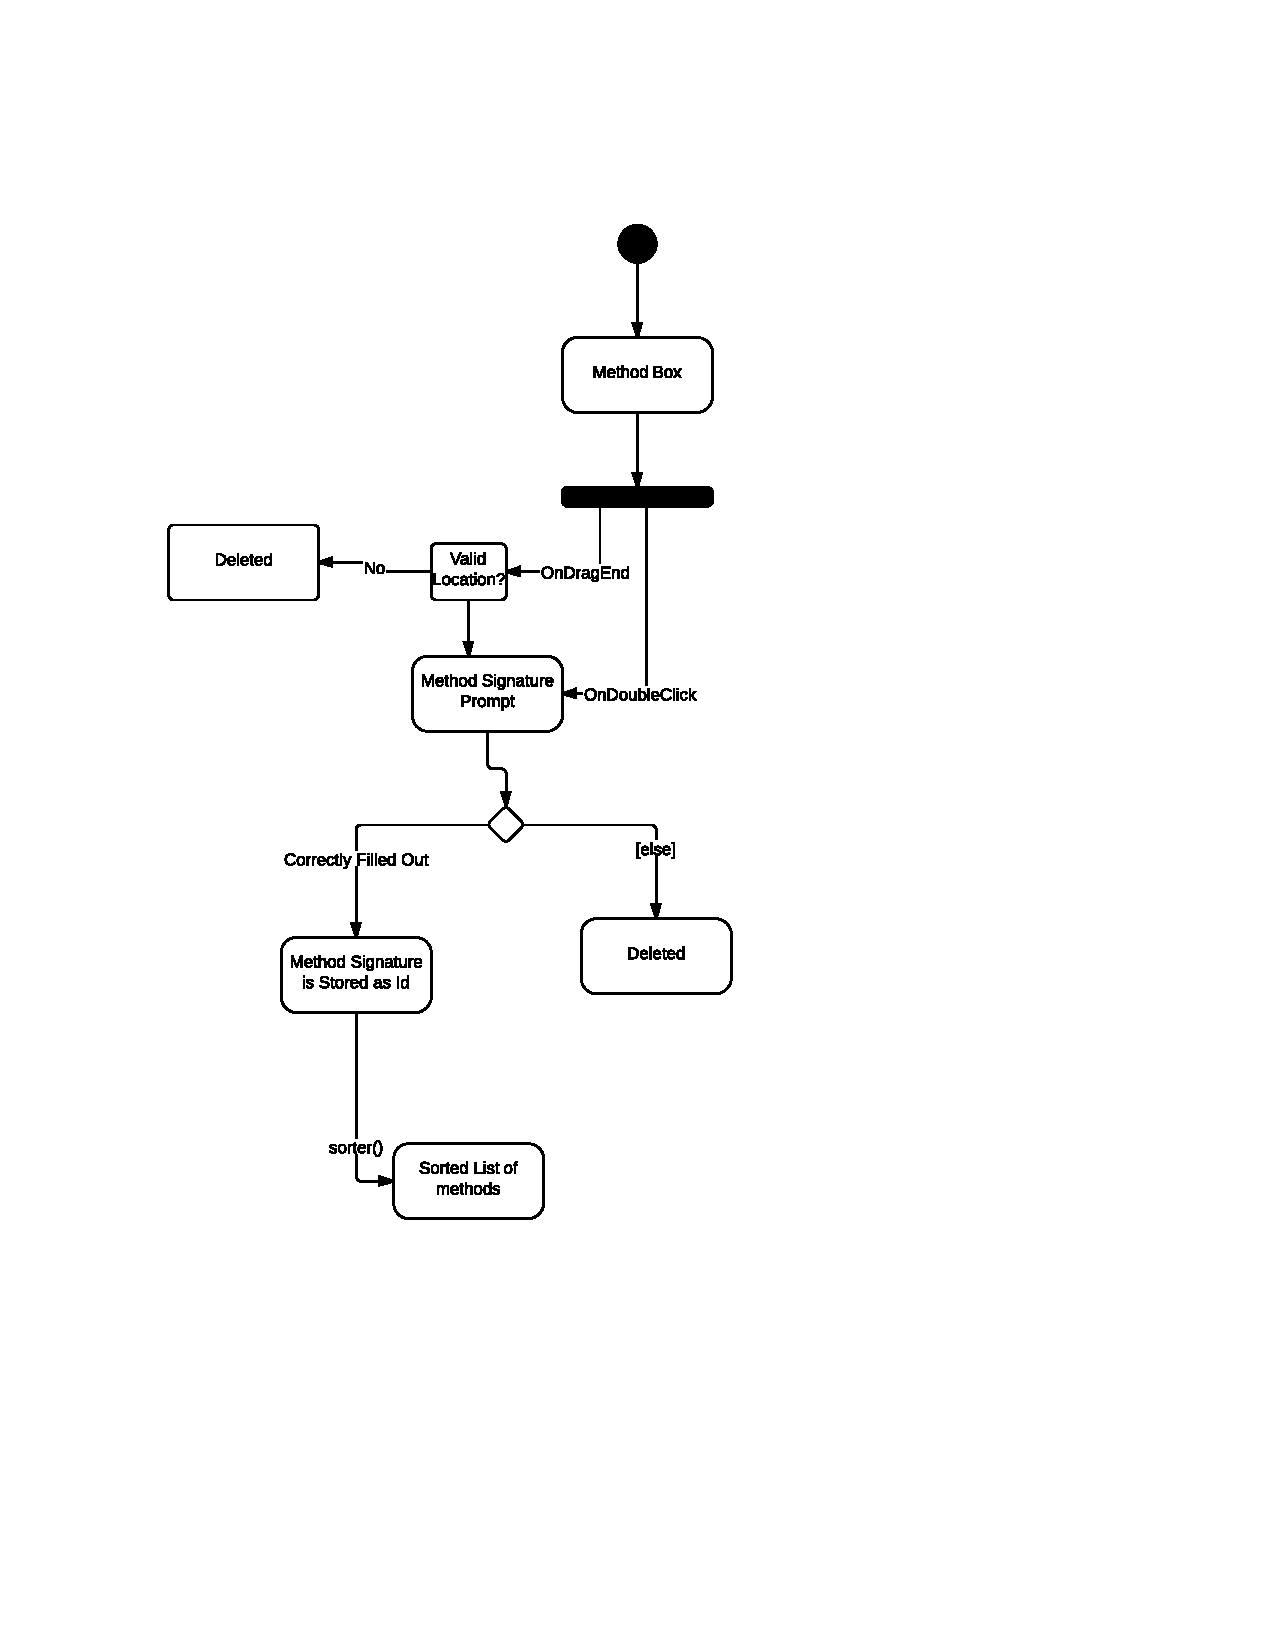
\includegraphics[]{methodBoxflow}
\end{figure}

\subsection{High Level Organization}
\subsubsection{Classes and Modules}
Canvas - The Visual Editor uses a KineticJS canvas. It serves as a layer for all blocks and ordering. All types of `Block' classes are placed on the same layer to ensure full control by the user. \newline \newline
Block Class - Blocks have certain types and functions. They can be dragged and dropped around the screen and are used for adding, editing, and sorting methods and elements in a user's story. To categorize blocks, we have placed them in three categories: Method manipulation, Animation functions, and Conditionals. For method manipulation (found in the method tab), a set of blocks are used for defining and ending new methods. Users can create an infinite number of new methods as long as they have enough vertical space on the canvas. For animation functions (found in the predefined tab), a set of blocks are predetermined from the Animation team API. We imported the methods the Animation team implemented and created a subsystem that keeps track of which `Sprites' are being controlled on the screen. Finally for the conditionals (found in the controls tab) are a set of blocks used for controlling classic conditional statements (if, for, while). These blocks are used by the user to create conditional events in their story.\newline \newline
Prompt Module - The prompt module displays messages and requires user input to define either numbers, variables, methods, or names for boxes. The 'Cancel' function on a prompt window will either revert a box back to original state if it was previously defined (i.e. double-click editing), or will remove the shape from canvas (i.e. dragend adding). The alert module notifies a user that they have entered an incorrect input, and allows them to change their input after clicking 'OK'. \newline \newline
Sorting Module - The sorting module keeps track of the order of all blocks in the visual editor and reacts differently depending on whether the user is trying to save their story or trying to load their story. While saving, the sorting modules write KineticJS objects in y-axis order into JSON text to be exported. While loading, the sorting module loads a previously saved JSON file and converts the JSON string into our KineticJS objects as Blocks.
See Figure 2 for a UML sequence diagram.
\begin{figure}[h!]
  \caption{A UML diagram of the sequence of the Visual Editor}
  \centering
	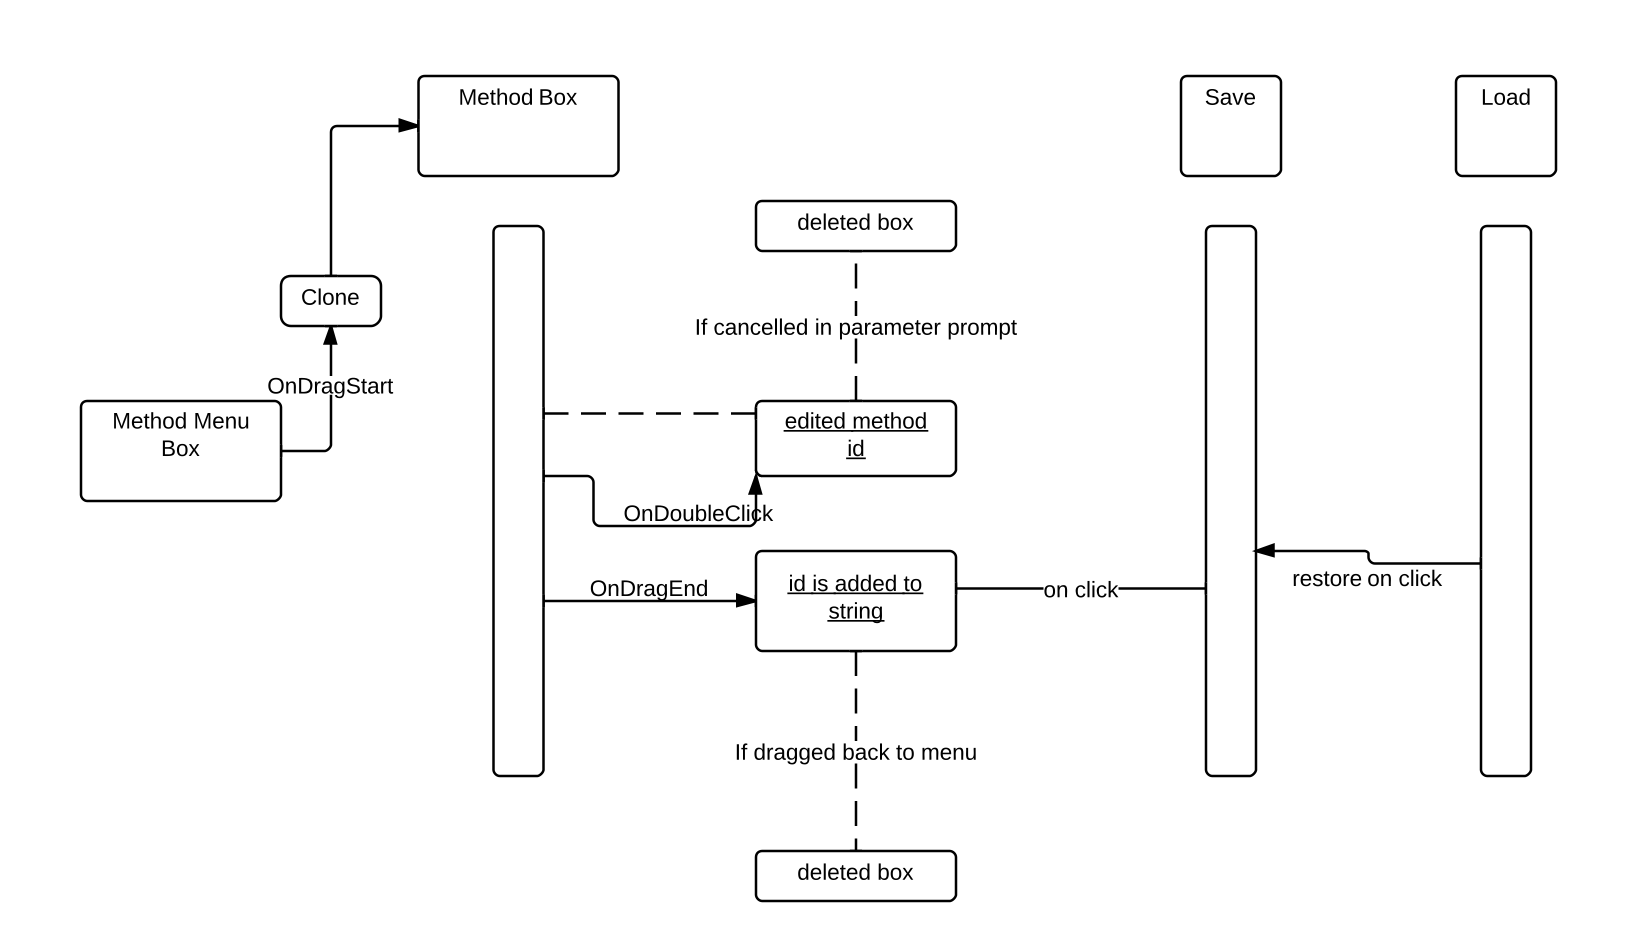
\includegraphics[width=\linewidth]{sequence}
\end{figure}

\section{Reflection: Vikram Nilakantan}
\subsection{Challenges}
\subsubsection{Technical Challenges}
The biggest technical challenge that I faced while on the Visual Editor team was my personal inexperience with the HTML5 Canvas or any of the graphical JavaScript libraries. After learning that the visual editor was going to be based in an HTML5 Canvas, I started to go through the process of figuring out how it worked and how to use it. I was told that the Canvas was very similar to doing graphics in Java, but since I had little to no experience with Java graphics, that advice did not help me as much. Two things mainly helped me overcome this challenge. The first was my prior experience using JavaScript and HTML. Even though the Canvas was unfamiliar, the language used to control it was very familiar and I was able to use my prior knowledge to accelerate the learning process. The second learning tool was simply trial-and-error. No one on the visual editor team had ever used the HTML5 Canvas or KineticJS before so what really helped us was several test documents trying to figure out how object were created and how we could interact with them. 
\subsubsection{Organizational Challenges}
Unlike other groups working on the Edith project, our group had six members, opposed to five. Since none of us had any familiarity with the technologies we were working with, our organizational challenges revolved around slow progress. Another challenge that surrounded the visual editor is that it was very difficult to separate work out until we had a solid foundation of what we were doing with Canvas and KineticJS and how we were going to execute such actions. Until we got to a point where we had a plan of action in which we knew how things were going to be done, we were unable to work separately and the only time progress was made was when all of us could meet up and surround one computer while we tried things out. Fortunately, we soon figured out what we were trying to do and were clearly able to divide tasks among group members.
\subsection{Applied Software Engineering}
Many aspects of the visual editor were designed and implemented according to software engineering techniques, however, I thought that the biggest lesson from software engineering we used was on creating the user interface. We estimated that the visual editor component of Edith is where the typical end-user would spend the majority of their time. Because of this, we wanted to spend some time on designing the user interface and become aware of exactly what actions users would be able to perform and make sure that certain elements of the editor are presented in a consistent manner.
\subsection{Different Approach}
One of the largest over-arching challenges that the visual editor team faced was that we were unsure of our requirements for the project and I felt like each of us had 'an idea' of what we were doing, but no one's ideas actually matched up with anyone else's. This posed a big problem at the beginning of this project and until we were sure of what we were doing, our progress stalled and at some points, came to a halt. If I were to do this project again, I would make sure that I was completely aware of the project/section requirements. If I were given more time to continue to work on this project, I would want to improve some of the graphical elements and transitions on the visual editor. The boxes and 'method containers' used currently are functional, but I feel like with more time, I could make those boxes more visually appealing. Another feature I would implement is ease-of-use for the end-user. That is, making sure it is clear how to operate the visual editor and making sure the user is not confused when they are trying to operate the application.
\section{Reflection: Graham Baker}
\subsection{Challenges}
Some of the main challenges I experienced during development were learning a new language, dealing with GitHub, and trying to find dividing lines between our group and others. I really enjoyed learning to use JavaScript. While it was pretty difficult at the beginning to work out how to access certain attributes, using global variables and other general points of confusion transitioning from traditional object oriented programming languages, I felt just pounding through trying to get my code to work was extremely beneficial and valuable. GitHub was also a source of confusion and frustration early on. I used the terminal for the first half of the semester and struggled to accomplish what I wanted to do. After I switched to the GitHub application, things got a lot easier. I am glad that I was introduced and got experience working with this important software development tool. Finally, the most difficult challenge this semester was settling on what each group was supposed to do. There were a few times where we were not really sure what we were supposed to be doing because our requirements overlapped with other groups. It was a good experience for us to have to grapple with the miscommunication and complexity that is so often the downfall of many projects. I learned that it is vital to get the requirements and direction of the project as early as possible to make life easier as the project goes on. 
\subsection{Applied Software Engineering}
The technique that I most frequently used over the course of the semester was the idea of iterative development. Since our requirements and goals were constantly shifting, we had to adapt every time we got a new direction. It was also nice to see that is consistent with how most software engineering firms operate. 
\subsection{Different Approach}
If we started over, I think we would probably seek out another graphics package to use for our user interface. While kinetic.js offered quite a bit of useful tools, I think one that supported text input would have probably suited our needs better. We landed on kinetic.js after trying to get things to work with jQuery UI as well as other graphics packages. As we approached the first implementation, we just had to go with kinetic.js. If we wanted to continue development we could find a better package that would suit our needs more appropriately. Now that we are at a decent position, I think there is a lot that could be done. It would be really great to add method box encapsulation like we wanted to do. Now that things are up and running, it is easy to see things that could be improved on and how to make the software easier to use for the user. 
\section{Reflection: Jessica Penick}
\subsection{Challenges}
\subsubsection{Technical Challenges}
I met a number of challenges in the entirety of this software engineering course, mostly due to the project itself. Firstly I spent the whole semester working intimately with languages that I had no previous familiarity with: JavaScript, LaTeX, and to some extent HTML (though I'd had a little past experience, and probably knew enough). I struggled with Git at first. For the most part it made sense conceptually, but using Git seemed to be an entire other story, and I one time deleted everyone's lab assignments on accident, which, luckily, could be undone due to the nature of the Git (that is, version control). It seemed like everyone got everything faster than I, which was, to say the least, frustrating. My group in particular had technical experience beyond mine, so I took on a supporting position to compensate. I read a bunch of resources on JavaScript, but I think I learned the most about the language from examining their code. Overcoming the challenge of LaTeX was a matter of online inquiries (read: Google), templates, and tutorials.
\subsubsection{Organizational Challenges}
The project some organizational challenges over the course of the project as well, both in the code and the group. For example, we never really designated a leader, which at first wasn't an issue, but later when disagreements arose proved problematic. We argued over which library to use, and later what functionality to focus on, but all of these came to peaceable ends, and never got particularly out of hand in the first place. The lack of a leader also lead to rather unsustainable agile module development on our part; often we would meet up then divide different tasks to each person to solve on their own, when I believe a pair system might have benefited us better in the long run. Even though pair programming is somewhat frustrating, two heads are, in fact, better than one. 
\subsection{Applied Software Engineering}
There was a lot to take away from this class, too. Chiefly process models, testing methods, architectural patterns, and design patterns. More notably, process models and testing methods were some of the applied techniques of our project. We prepared and implemented a plan-driven development, but I think in the end our project, and more specifically my group's module in it, became a kind of agile development process, which isn't necessarily a bad thing; both models have advantages and disadvantages. Testing, too, played an instrumental part in development. Of course testing should always be instrumental, but linting the code proved especially important since clean code is easier to parse and revise later.
\subsection{Different Approach}
If we were to start over, I would do a few things differently: 1) I'd choose a group I could be more helpful in, 2) I would be more involved in the coding process, or, barring that, I'd have taken more of a stand on the organization of the code/communication within and without the group. There is more to do than coding in a development team, so I would have operated in a position of administration rather than facilitation. If we were to continue developing the code, I would work to optimize it for efficiency—-maybe make it more easily maintainable. That includes documenting it thoroughly, observing the interfacing between modules and seeing how them may be improved by the reallocation of responsibilities, or standardization of the information being passed around. Mostly re-imagine it as a project conceived as a single idea from the top down (or more likely, the bottom up). Also, over time, add more features, clean up/unify the interface, and generally expand it (maybe a message board to discuss created stories, or the ability to annotate them? Possibilities are endless).
\section{Reflection: Eli Spiegel}
\subsection{Technical and organizational Challenges}
The project started trying to use the waterfall method, however as it progressed the lack of direction made the waterfall method challenging. This led to our team and a few others moving to a more agile approach. Agile helped us get a product that worked in a shorter amount of time as we were able to progress and find different problems instead of spending all of our time planning and then quickly finding new issues. Other issues included communication between people with diverse schedules, and working with tools and languages I was unfamiliar with, mostly JavaScript and GitHub.
\subsection{Starting this Project Over}
I think writing requirements as a class with Joel as the ``client" could have made for a better use of the waterfall method as everyone would have a better understanding of the overall project, which would help with moving forward on the individual modules and solve division of labor/dependency issues. Another issue the project had was a lack of experience with the languages/tools groups would be using took the focus off of the software engineering problems and made them more implementation problems. I believe that a stronger focus on learning the tools and languages at the start of a project will make it clear what problems may arise and possible ways to solve them. 
\subsection{Learning}
In the end some of the more valuable things I learned were how to write code as a group, and how to use tools such as GitHub. I also learned that knowledge is the most important tool in software development. If a group comes in knowledgeable about the tools and about what the goal is that they will build even complex projects in a fairly short amount of time.
\section{Reflection: Walker Bohannan}
\subsection{Challenges}
Developing the Visual Editor platform for the Edith project involved a tremendous amount of work, and creating boxes with which to create and edit code with was not without its difficulties. Some specific challenges that I encountered in the beginning were on deciding which framework to use. Some options we considered were jQuery UI, RaphaelJS, finally settling with KineticJS, which offered the tools to manipulate what we needed to on a HTML5 canvas. Organizational issues often arose with cross-team integration of using GitHub, and resolving conflicts was not always as simple as we might have hoped. In the end, we figured out how to solve these problems, and came away from the problems with renewed expertise and troubleshooting skills regarding GitHub. That being said, I was always extra careful of any changes I made when pushing to Git, and being sure if I needed to modify another group's code I was explicit in what I did and commented my changes so they would not be deleted. Another challenge that required being overcome was a mid-project reassessment of what our role in the project as a whole was. Our requirements were not explicit until this point, and until then there was a lot of, ``well the other group is taking care of that," going on not just in our group but in others as well. Other challenges were learning a new language - JavaScript, which I knew none of prior to this course. The syntax quickly came in, and past coding experienced helped, and soon I was enjoying using a new language as I had used others, which only minor hiccups along the way.
\subsection{Applied Software Engineering}
A software engineering technique that helped us during the process was using rapid application development, where we constructed prototypes, and would test them (lining up with the deadlines for our integration tests). We iteratively developed our prototypes. We also fulfilled one of the main principles of rapid application development by emphasizing the ``business need," which was being able to create and write code using blocks rather than focusing on the technological excellence. We used ourselves to act as the users, testing continuously. In continuity with our integration deadlines, we focused on reducing implementations and making our deadlines with what we had working well. Another useful technique was to use pair programming, or even group programming, with one person ``driving" while the other members looked on. This was especially useful in imparting knowledge of JavaScript (which started at zero), as we started this project. We would switch roles often, with different combinations of different group members taking different roles, so nearly everyone had a chance at the controls.
\subsection{Different Approach}
If I were to start this project over again, I would probably create my own framework, rather than use KineticJS or something else similar to it. Creating our own framework would enable us to manipulate objects and variables in a way that was efficient and could be used in a way to how we could optimize it. Often I felt as though I was spending a majority of the time figuring out how to make the KineticJS work, figuring out correct syntax rather than being able to go through my code and edit and implement new features. That being said, having the KineticJS framework probably did save us an enormous amount of time, rather than discovering halfway through the project that our own implementation was not going to work. As far as continuing work using the existing code we have, I think method encapsulation would be the next step, as well automatic end bracket creation. However, with how we are implementing it, I think requiring the user to add end brackets is a very relatable aspect of coding, and will teach the user how to code better. That being said, implementing a ``compile" function, letting the user know they forgot something syntactically would also be useful.
\section{Reflection: Steve Marx}
\subsection{Challenges}
Two different types of challenges were encountered in the project: technical and organizational. The most obvious hurdle from a technical perspective was the need for the entire team to learn multiple new languages/tools quickly, concurrent with the start of a complex project. New technologies included Javascript and the various frameworks (JQuery, KineticJS, etc.) that could provide functionality to the Visual Editor module, Git collaboration and HTML, among others. Some of the Javascript libraries would work better for particular aspects of the module, but selection was difficult due to the team's collective inexperience with them. The technical challenges were overcome through excellent determination, self-education and trial and error by VE team members. My most important technical take-aways are Git use and general Javascript knowledge.
Although Edith is obviously a technical project, organizational challenges seemed to be even more important than technical challenges. It was a good simulation of projects outside of the classroom, in which a person or team is given a task and a completion date and left to accomplish the goal in a mostly self-directed way. However, in some ways it was more challenging. For example, in a company, individuals, teams, and the entire project would have clearly defined roles and management/leadership relationships (as well as likely having more experience with the technical aspects). Projects need managers and technical contributors and some who can fill both roles. At some point in the project, the class started to see the need for more defined roles and coordination among groups, and assigned a designated contact person for each team. That was just one example of a positive adaptation, and I am sure that if today the class were given another project based on the same languages, it would be done much more effectively. You can only learn through experience, and I definitely have a better idea of how large software projects work in large groups, and how I could improve my performance.
\subsection{Applied Software Engineering}
Software engineering techniques were applied both formally and informally. The most helpful formal use was the creation of the Requirements Specification, including the functional requirements, use cases, UML and non-functional requirements. Although the project still required some changes to teams' understanding of their roles, this document forced the team to be specific about its objectives and served as a guide to development. In general, Visual Editor development was done through an iterative prototyping methodology in which several team members developed different ways to structure the module. Of course, there was duplication of efforts in the early stages, but ultimately the method produced a common platform for everyone to work from. Testing methodologies, including static analysis software, was also helpful. 
\subsection{Different Approach}
It is easy to look back and come to the conclusion that you could have done things differently, but is it a useful exercise? I think it is. In my last corporate position, all company divisions were transitioning to a new way of financial reporting. Each quarter, the managers of each division gathered for a ``post-mortem" to review what went wrong (and right) with the project that quarter. It was a great chance to share issues with upper management and learn from the successes and challenges of other groups, too. On the Edith project, I would have devoted much more energy in the beginning to ensuring that teams understood their roles in every respect - generally; specifically; the interactions with other modules and teams, etc. In the early weeks, it would have been helpful to spend days at the chalkboard with the whole class present, diagramming out exactly who was doing what - sketches of module appearances, and clear discussion of where one team's module would end and the next team's would begin (including discussion of what would need to be passed from team to team). Confusion over these issues hindered our progress nearly throughout the project and resulted in new roles and confusion essentially through completion. There were many discussions of roles, but they were in the form of conversations between individuals (while many assumptions were made by all the groups - ``I think Team X is doing that") and communication was not formalized and widely distributed. If we were to continue developing the Visual Editor module, we would have some more time to focus on the user's learning experience. For example, help boxes and coding tips (e.g., how to use if statements) would be provided for the user. In addition, blocks could be shaped to fit together in logical (allowed) ways for programming, similar to the blocks of Scratch. 
\section{Glossary and References}
Alice - educational software that teaches students programming in a 3D environment. http://www.alice.org/index.php \newline \newline
Git - a distributed revision control and source code management (SCM) system with an emphasis on speed. \newline \newline
HTML5 - a markup language used for structuring and presenting content for the World Wide Web. \newline \newline
IDE - Integrated Development Environment - software application used for software development \newline \newline
jQuery - fast, small JavaScript library. It makes things like HTML document traversal and manipulation, event handling, animation, and Ajax much simpler with an easy-to-use API that works across a multitude of browsers. jQuery.com \newline \newline
JSON - JavaScript Object Notation. A lightweight data-interchange format. \newline \newline
KineticJS - HTML5 Canvas JavaScript framework that enables high performance animations, transitions, node nesting, layering, etc. http://kineticjs.com/ \newline \newline
RAD - Rapid Application Development. Software development methodology that uses minimal planning and extensive prototype development. \newline \newline
regex - Regular Expression. Sequence of characters that forms a search pattern, mainly for use in pattern matching (Edith uses to verify proper user input) \newline \newline
Scratch - educational software that teaches students programming in a 2D environment http://scratch.mit.edu/ \newline \newline
Sprite - 2-dimensional image or animation (a character) \newline \newline
\end{document}

